\chapter{Approximating Type Stability Statically}\label{chap:approx}

\lstset{language=julia}

% \paragraph{Plan of attack}
% \begin{enumerate}

% \item
% Inferring type stability versus inferring types

% \item
% Method: Using Julia's built-in type inferencer to approximate type stability.

% \item
% Basic algorithm
% - flowchart, main steps, running example

% \item
% Enumerating concrete subtypes

% Meta: features of the algorithm I'd like to discuss at some point.
% - Corner cases, termination, fuel.
% - Limitations: incompleteness and unsoundness.
% - Relation to Julia subtyping.

% \item
% Search space explosion
% due to under-constrained types, e.g.:
% - ''fat'' (i.e. many subtypes) abstract types like Any
% - unbounded existentials
%
% We propose three approaches to fight this problem:
% - fuel
% - run type inference with Any: concrete result means it's stable
% - the types DB idea

% \item 
% Implementation
% - User's API (macro and otherwise)?
% - Processing Julia modules: pitfalls and workarounds.

% \item
% Evaluation
% - Results on 10 popular Julia packages.


% \end{enumerate}

Chapters~\ref{sec:empirical} and~\ref{sec:jules} consider type stability as it
relates to program \emph{execution}: chapter~\ref{sec:empirical} analyzes the
state of Julia's virtual machine after running package test suites, and chapter~\ref{sec:jules} models a
type-specializing just-in-time compiler that executes at run time.
In this chapter, I set to approximate the property of type stability for
arbitrary Julia code statically, without running the code in question.
I focus only on type stability but not type groundedness because,
as discussed in~\chapref{sec:jules}, groundedness is enabled by calling
type-stable API.
% \paragraph{Note on Dropping Type Groundedness.} It turns out that attempts to
% infer type groundedness statically fail fast: this is too low-level of a
% notion requiring us to reason at the level of intermediate representation, and at
% that level, precision gets lost very fast. The good news is that, as we learned
% in~\chapref{sec:jules}, type groundedness is enabled by calling type-stable
% API, so being able to provide such API should be enough for a careful client.
% Therefore, in this chapter we focus on analyzing type stability of methods, and
% leave type groundedness off.

\section{Inferring Type Stability versus Inferring Types}

Explaining my approach to infer type stability requires a definition of stability.
So far, I approached the definition twice: informally
in~\ref{ssect:ts-informal} and formally in~\ref{sec:stability-formal}.
The original informal
definition does not take into account the distinction between concrete and
abstract types: using this loophole, any code can be declared type stable
because it is always possible to ``predict the type of the output'' as \c{Any}.
Building upon the formal definition (that does acknowledge the distinction
between abstract and concrete types)
I provide another informal definition to explain intuitions behind this
chapter.
\begin{definition}[Type Stability, Informally]
  A Julia method is called \emph{type stable} if, for any concrete type of the
  input, it is possible to infer a concrete type of the return value.
\end{definition}

A natural idea for inferring type stability in Julia would be to formulate it as
a forward static analysis: being an abstract or concrete type is one bit of
information that has a known value at the input (concrete) and should be
propagated to the output, possibly changing on the way.

To test the static analysis idea, consider a positive example first: the
identity function.
% TODO: there's a weird break in the listing near page break (see PDF)
\begin{lstlisting}
  function id(x)
    x
  end
\end{lstlisting}
%
It is straightforward to infer that, given any concrete input type, the return
value is also concretely typed: the one bit of information carries over to the
result in one step.

However, another example---the increment function---shows that the task quickly 
becomes unwieldy.
%
\begin{lstlisting}
  function inc(x)
    x + 1
  end
\end{lstlisting}
%
Concreteness of the result returned by \c{inc} depends on concreteness of
the result of the call to \c{+}. In turn, the property of the return type of
\c{+} depends on which \c{+} method Julia will dispatch to at run time.
There are about two hundred method implementations of \c{+} in the standard
library alone, and packages add more. Some of those methods are type stable
(e.g. \c{+(::Int64,::Int64)}), and some of them are not (e.g.
\lstinline|+(::Rational{Bool},::Rational{Bool}|)
\footnote{%
  The reason for the
  \c{+(::Rational\{Bool\},::Rational\{Bool\})} method to be type
  unstable is not important, but in a nutshell, Julia has made a questionable
  design decision about the return type of \c{{+}(::Bool,::Bool)}, which in the
  current implementation is \c{Int}
  (see discussion \url{https://github.com/JuliaLang/julia/issues/19168}),
  and when adding two rational numbers with boolean components, depending on the
  values of the summands, you get back either \c{Rational\{Bool\}} or
  \c{Rational\{Int\}}.}
).
Therefore,
to infer the property of interest, in general,
we need to predict which methods are selected at run time.

The \c{inc} example shows that inferring type stability of Julia code
requires
reasoning about %which methods will be called at run time, % repetition of prev sentence
%which, in a language with dynamic dispatch, leads
multiple dynamic dispatch, which leads
to reasoning about the \emph{types} of intermediate values rather than only
the concreteness bit. But if there was a tool for computing type information
beforehand, a special-purpose analysis for type stability would not be needed: 
it suffices to ask the tool for the type of the return value and
check if that type is concrete. 
%The observation of interactions between type
%stability and type inference can be formulated
This observation leads to the following conjecture:

\begin{conjecture}
  Inferring type stability of a Julia method statically is no easier than
  performing type inference of that method.
\end{conjecture}

A complete type inference algorithm would allow for checking type stability of
Julia code. But should type inference be implemented from scratch? There are two reasons to
not go this way.
\begin{enumerate}

  \item It is not clear that inferring types for source-level Julia code
  %typing Julia 
  without changing anything in the language
  can yield a meaningful result (more on this see~\cite{Chung23}).
  For instance, in the \c{inc} example, a sound return type cannot be
  much better than \c{Any}.

  \item Julia already has a built-in type inference engine, which 
    was modeled as a black box in~\chapref{chap:jules}. 
    This engine is used for code optimizations. 
    Thus, analyzing type stability based on a custom type inference 
    algorithm 
    %to infer types and analyze type stability 
    can produce results that diverge from Julia, misleading the users
    about potential optimizations.
    %our results may diverge from Julia's. 
    This would be of limited usage for Julia users.
\end{enumerate}

\section{An Algorithm To Infer Type Stability}%
\label{sec:approx:algo}

\subsection{High-Level Description}
\label{ssec:algo:high}

If our predictions for type stability are to align with the Julia
implementation, the analysis should closely model Julia's run-time behavior,
as described in~\chapref{chap:jules}. The type-specializing JIT-compiler
from~\chapref{chap:jules} makes optimization decisions based on \emph{concrete
  input types} with the help of Julia's type inference engine. 
Therefore, the algorithm for
predicting these decisions statically considers all (or as many as possible,
see~\secref{sec:approx:space}) allowed concrete input types of a method.
\figref{fig:infer-ts} describes this algorithm at a high level.

\begin{figure}
  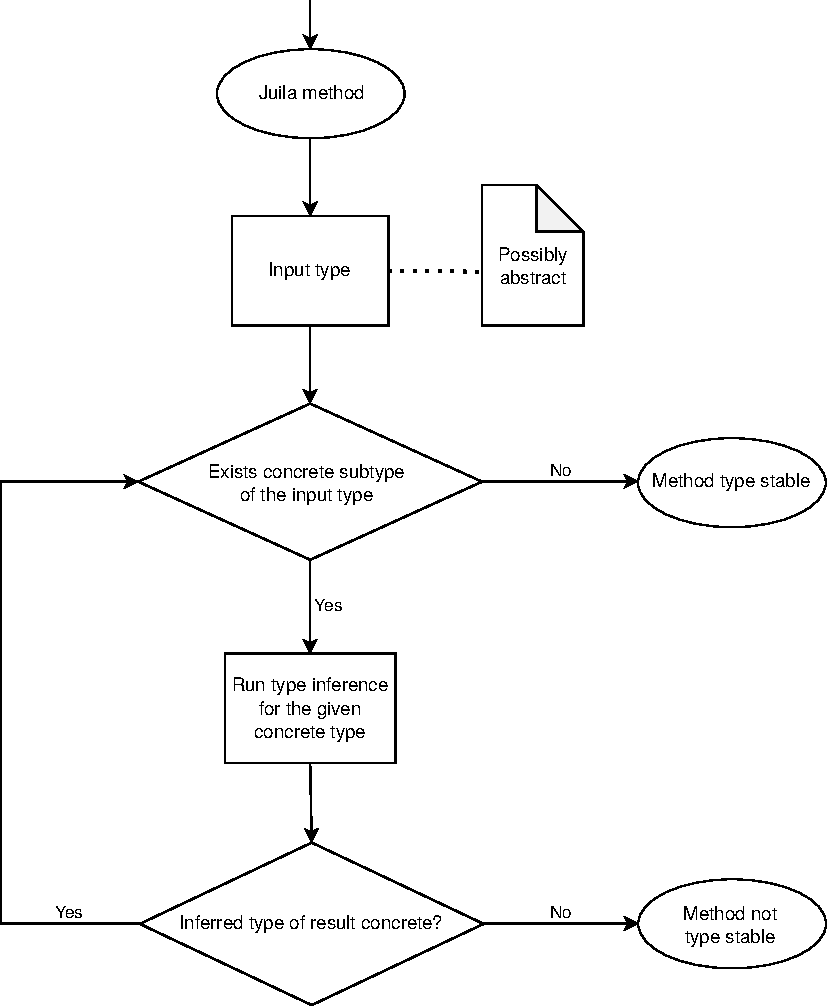
\includegraphics{figs/infer-ts.pdf}
  \caption{Inferring type stability of a Juila method}%
  \label{fig:infer-ts}
\end{figure}


Let us consider every step of the algorithm described
on~\figref{fig:infer-ts} and explain its meaning using an example.
The list below also assigns the numbers to each step in the algorithm.
\begin{description}

  \item[Step 1] The input of the algorithm is a Julia method. Methods in Julia are
  represented by run-time objects of type \c{Method} and can be manipulated as
  all other objects (e.g. stored in collections, responding to field accesses, etc.).

  For example, consider the \c{length} method from Julia's standard library. We can
  get the corresponding \c{Method} object using the standard \c{@which} macro
  applied to an application of the \c{length} method. This can be done in the
  Julia REPL (signified by the \texttt{julia>} prefix).

\begin{minipage}{.92\textwidth}
\begin{lstlisting}[style=jterm]
  julia> @which length([1,2,3])
  length(a::Array) in Base at array.jl:215
\end{lstlisting}
\end{minipage}

  The output shows that the given \c{length}-call will dispatch to the
  method defined in the \texttt{Base} module (Julia-speak for the standard
  library). The output also shows the location of the method in the
  standard library and, most importantly for us, the signature of the
  method. In fact, what we see here is a pretty-printed representation of
  the \c{Method} object representing a particular Julia method.

  \item[Step 2] The first task of the algorithm is to get the input type of the given
  method. This is possible through querying the \c{sig} field of the method object.

  Building on the example above, we can get the signature of the \c{length}
  method as follows:

\begin{minipage}{.92\textwidth}
\begin{lstlisting}[style=jterm]
  julia> m = @which length([1,2,3]);

  julia> m.sig
  Tuple{typeof(length), Array}
\end{lstlisting}
\end{minipage}

  A signature of a method %will usually have 
  contains the special singleton function
  type (\c{typeof(...)}) as the first component, and the rest is (easy to
  convert to) the type of the input --- an $n$-tuple. In this example, the type of
  the input is 1-tuple, consisting of the existential array type
  \c{Array\{T, N\}\ where T where N} abbreviated simply as \c{Array}\footnote{%
A user can always look under the abbreviation using the \c{dump} function.
%:
% \begin{lstlisting}[language=julia,style=jterm]
%   julia> dump(Array)
%   UnionAll
%     var: TypeVar
%       name: Symbol T
%       lb: Union{}
%       ub: Any
%     body: UnionAll
%       var: TypeVar
%         name: Symbol N
%         lb: Union{}
%         ub: Any
%       body: Array{T, N} <: DenseArray{T, N}
% \end{lstlisting}
}.

  \item[Step 3] The input type can be either concrete, which, in Julia, means that there can
  be no proper subtypes of that type, or abstract. In either case, the choice on the
  current step will enter the loop at least once, because for concrete input type,
  the check holds once trivially (e.g.\ there is exactly one concrete
  subtype of the concrete type \c{Int} --- it is \c{Int} itself).

  If the input type is abstract, we need a procedure enumerating all concrete
  subtypes of it. An implementation for this procedure is discussed below
  (\ssecref{sec:approx:enu}), but it suffices to
  treat is as a black box for now.

  In the case of the \c{length} method, the input type, \c{Array}, is
  an existential type and hence abstract. Therefore, the enumeration procedure
  should have yielded a concrete subtype of \c{Array}. Assume that
  the concrete type is \c{Array\{Float64, 1\}}.

  \item[Step 4] Running Julia's type inference for a given method and a given concrete input
  type is done by calling Julia's standard \c{code\_typed} function.
  The only issue with the function is that it expects a function object as a
  part of the input, not a method object. But getting from a method to the
  corresponding function is possible using the signature field discussed above,
  and, in particular, the singleton function type contained in the first component
  of the \c{sig} field: accessing the single function object using the function
  type is possible via the \c{instance} field.

  Running type inference for the \c{length} method and the concrete input type
  \c{Array\{Float64, 1\}} could be done as shown on \figref{fig:julia-type-infer}.
  The return value is an array of \c{CodeInfo} objects that represent
  the type-annotated method bodies of all methods that a call with the given input type
  could dispatch to (for a concrete input type and no ambiguities in method
  definitions, the resulting array always contains exactly one element).
  Method bodies are transformed into
  a lower-level intermediate representation, similar to the one
  discussed in \ssecref{ssec:perf} and \chapref{chap:jules}. 
  In the running example, the
  method body contains a single call to an intrinsic Julia function that is
  known to return a value of type \c{Int64}.

  \begin{figure}[hbt]
% \begin{minipage}{.92\textwidth}
% \begin{verbatim}
\begin{lstlisting}[style=jterm]
  julia> code_typed(m.sig.parameters[1].instance,
                    (Array{Float64, 1},),
                    optimize=false)
  1-element Vector{Any}:
   CodeInfo(
  1 - %1 = Base.arraylen(a)::Int64
  +--      return %1
  ) => Int64
\end{lstlisting}
    \caption{Running Julia's built-in type inferencer}%
    \label{fig:julia-type-infer}
  \end{figure}
% \end{verbatim}
% \end{minipage}

  \item[Step 5] Concreteness of the inferred return type is checked 
  with the standard Julia \c{isconcretetype} predicate. 
  In the running example, for the concrete input type \c{Array\{Float64, 1\}},
  the return type of \c{length} is inferred to be \c{Int64}, which is a concrete type.
  Following the second decision element on \figref{fig:infer-ts}, we get back to
  the start of the loop and try another concrete subtype of the input type,
  if there is any.
\end{description}

There are two main auxiliary procedures that the algorithm relies on: enumeration of
concrete subtypes of a given input type and type inference over a method with the
given input type. The latter can be fully outsourced to Julia itself, while the
former requires separate consideration.

\subsection{Enumerating Concrete Subtypes}%
\label{sec:approx:enu}

\subsubsection{Julia's \c{subtypes} method}

On \astep 3 of the algorithm (\ssecref{ssec:algo:high}), we need to generate a
concrete subtype of the input type. This task does not have a direct
implementation in Julia's standard library. The closest counterpart that Julia
provides is the \c{subtypes} method to query declared subtypes of a given
nominal type. For example,
\begin{figure}[h]
\begin{minipage}{.49\textwidth}
\begin{lstlisting}[style=jterm]
julia> subtypes(Signed)
6-element Vector{Any}:
 BigInt
 Int128
 Int16
 Int32
 Int64
 Int8
\end{lstlisting}
\end{minipage}
~
\begin{minipage}{.49\textwidth}
\begin{lstlisting}[style=jterm]
julia> subtypes(AbstractSet)
5-element Vector{Any}:
 Base.IdSet
 Base.KeySet
 BitSet
 Set
 Test.GenericSet

\end{lstlisting}
\end{minipage}
\end{figure}

The challenge here is that Julia's subtype relation is richer than the
nominal type hierarchy. For example, if a method declares the type of its input
as
\begin{lstlisting}
  Union{AbstractSet, AbstractRange}
\end{lstlisting}
then the method can be called with an argument of type \c{Set\{Int\}}, and,
therefore, it should be possible to discover such a type following the algorithm
on~\figref{fig:infer-ts}. However, it is not possible with the \c{subtype} method alone:
from \c{subtypes}' point of view, the union type above has no subtypes:
\begin{lstlisting}[style=jterm]
  julia> subtypes(Union{AbstractSet, AbstractRange})
  Type[]
\end{lstlisting}
(the query returns an empty array of elements of the type \c{Type}).
Therefore, structural types %that have special subtyping rules, like 
such as unions,
tuples, and existential types, need a special treatment.

The \c{subtypes} method does not cover the whole subtyping relation not only
because it cannot work with structural types but also because it is limited
to direct declared subtypes. For example, in the subtype chain
\c{Int <: Signed <: Integer}, \c{subtypes} reports only \c{Int <: Signed}
and \c{Signed <: Integer} but not \c{Int <: Integer}. Thus, we have to build
the transitive closure manually.

In the following subsection, I show how to generalize the \c{subtypes}\!\!method to
a method I call \c{direct_subtypes} that produces direct subtypes for a Julia
type of any form. Then, the transitive closure mentioned above can be
obtained by iterating \c{direct_subtypes} applications,
starting from the signature of a method we are checking for
type stability.

After generating all subtypes of a given type, it is possible to filter for concrete
subtypes using the built-in Julia predicate \c{isconcretetype}. This completes
the task of enumerating concrete subtypes and the description of the algorithm
as presented on \figref{fig:infer-ts}.


\subsubsection{Enumerating Direct Subtypes}

My goal in this section is to define a general utility generating direct subtypes of a given
type, which I call \c{direct_subtypes}.
% \begin{lstlisting}
%   const JlType = Any   # type synonym
%   function direct_subtypes(t :: JlType) :: Vector{JlType} ...
% \end{lstlisting}
This is done by case analysis on the existing Julia kinds (i.e., types of types)
and expressed with multiple methods
of the \c{direct_subtypes} function. The implementation largely follows from the
description of Julia's subtyping relation given in~\cite{oopsla18b}.

The \c{direct_subtypes} utility can be defined, for the most part, via multiple dispatch
using Julia's kind system.
The only special sort of types that does not have a dedicated kind is the tuple type.
In particular, although tuple types fall under the \c{Datatype} kind,
the standard \c{subtypes} method cannot help with tuple types as much as it can with user-defined datatypes.
For example,
both \c{Integer} and \c{Tuple\{Integer, Integer\}} are datatypes, but
\c{subtypes} returns an empty array of types for the latter.

%
% good for the Background section, perhaps?
% Generally, every Julia type is
% either a union type (kind \c{Union}), an existential type (kind \c{UnoinAll}) or
% a datatype (kind \c{DataType}), for example:
% \begin{lstlisting}[style=jterm]
%   julia> Union{Int, String} isa Union
%   true
%   julia> Vector isa UnionAll
%   true
%   julia> Int isa DataType
%   true
% \end{lstlisting}

% Overall,
% some special types, notably tuple types, fall under the datatype kind. Still,
% existing kinds other than \c{DataType}, are useful.

\begin{description}

  \item[Union Types]
        Unions in Julia have the kind \c{Union} and a form of \c{Union\{A,B,C\}}
        with arbitrary number of arguments \c{A, B, C}.
        Direct subtypes of \c{Union\{A,B,C\}} is the following list of types: \c{[A,B,C]}.

  \item[Existential Types]
        Existential types in Julia have the kind \c{UnionAll}\!\!and a form of
        \c{t where T}, e.g. \lstinline|Vector{T}| \c{where T}, commonly abbreviated as \c{Vector}. Every
        \c{where}-bound type variable has associated upper and lower bounds with
        default values \c{Any} and \c{Union\{\}} (the top and bottom types),
        respectively. Direct subtypes of an existential type are all
        instantiations of its variable allowed by the bounds. In particular, we
        need to compute all subtypes of the upper bound, filter out those not
        satisfying the lower bound, and use the resulting set of types to
        instatiate the variable with.

        For example, consider the \c{Vector\{T\}} \c{where T<:Signed} type.
        All subtypes (not only direct or concrete) of \c{Signed} are:
        \c{BigInt, Int128, Int16, Int32, Int64, Int8}. Therefore, all direct
        subtypes of the vector type in question are:

\begin{minipage}{.92\textwidth}
        \begin{lstlisting}
Vector{BigInt}
Vector{Int128}
Vector{Int16}
Vector{Int32}
Vector{Int64}
Vector{Int8}
        \end{lstlisting}
\end{minipage}

        % TODO / Note for a curious reader: there are two ways to subtype
        % existentials around abstract parametric types, e.g.
        % AbstractArray{T} where T have two groups of subtypes:
        % - AbstractArray{Int, 1}, etc.
        % - Array, etc.
        % so, one group is due to the structural properties of the existential,
        % and the other one is due to nominal hierarchy.

  \item[Datatypes]
        In general, non-parametric nominal types defined using the \c{primitive} (e.g. \c{Int64}) or
        \c{struct} (e.g. \c{Pair}) qualifiers,  can be processed
        using the \c{subtypes} method (see examples in the previous section).%:
        These also include fully-instantiated parametric types
        (e.g. \c{AbstractSet\{Int\}}).

  \item[Tuple Types]
        Tuples play a key role in method dispatch because method
        %with more than one argument have 
        signatures and arguments are represented with tuple types. As the \c{subtypes} method
        cannot work with tuples (for any input tuple, it returns an empty
        array), tuple types are unfolded according to the following rule:
        \begin{itemize}
          \item direct subtypes of the 0-tuple type is an empty set;
          \item direct subtypes of a 1-tuple type are 1-tuples of the direct 
          subtypes of its single type argument;
          \item direct subtypes of an $n$-tuple type are a Cartesian product of
          direct subtypes of its first component and direct subtypes of the last
          $n-1$ components.

          For example, for an abstract type \c{A} with exactly two declared
          subtypes \c{B} and \c{C}, the set of direct subtypes of
          \c{Tuple\{A,A\}} is

\begin{minipage}{.9\textwidth}
        \begin{lstlisting}
Tuple{B,B}
Tuple{B,C}
Tuple{C,B}
Tuple{C,C}
        \end{lstlisting}
\end{minipage}

        \end{itemize}

        % % TODO: This section is to be moved to the discussion of state space size.
        % % General idea (which is not yet expressed in this text) is that we
        % probably don't want to enumerate all singleton types.
  % \item[Special Singleton Types]
  %       In Julia, every type with a single instance is called singleton type.
  %       If it is a regular user-defined type (like \c{Val} from the standard
  %       library), then it can be processed using the general strategy described
  %       above (as a datatype or an existential type, depending on its form).
  %       But two
  %       kinds of Julia values has special singleton types:
  %       \begin{itemize}
  %         \item Every function has a dedicated \c{typeof}-type (e.g. the
  %         function \c{sum} has the type \c{typeof(sum)}). The \c{typeof}-types
  %         are concrete and therefore have an empty set of proper direct
  %         subtypes. There is a common supertype for all function types called
  %         \c{Function}. It does not
  %         \item Type objects have \c{Type{T}} types (e.g. \c{Int} has the
  %         \c{Type\{Int\}} type). These types
  %       \end{itemize}
  %       primitive values can be used as arguments of
  %       parametric types (e.g. )

\end{description}

\section{Search Space and Approximation}%
\label{sec:approx:space}

The algorithm as presented on \figref{fig:infer-ts} is an instance of a tree
search algorithm: it traverses the subtype tree starting from a given node and
tries to find a leaf on the tree that violates a given property. The nodes of
the tree are discovered dynamically---using the \c{direct_subtypes} utility.
%
With the grammar of types and subtype relation as rich as Julia's, the search
may diverge. In this section, I show how to control the search space of the
algorithm.
% TODO: mention that limiting the search space means we don't get an exact
% answer anynmore -- hence, approximation.

\subsection{The Problem: Underconstrained Types}%
\label{ssect:uconstr-types}

There are several groups of abstract types that have ``too many'' subtypes to explore
and, therefore, lead to issues with the subtype tree exploration; I call such
types \emph{underconstrained}. Most common groups of underconstrained types are
as follows.
\begin{enumerate}

  \item Nominal types declared close to the top of the subtype lattice
    have too many (even if finite) concrete subtypes to explore in a reasonable time.
    The most prominent example is the top type (\c{Any}) itself.
    The top type in Julia 1.8 standard library has 567 direct subtypes, most of
    which are abstract and, therefore, have a number of direct subtypes of
    their own, etc., so it is not feasible to track the whole tree during the search.

  \item Existential types whose variable's upper bound is an underconstrained
    type. Especially large search space is produced by existentials with \c{Any}
    as the upper bound (\emph{unbounded existentials}, for short).
    Note that out of the 567 direct subtypes of \c{Any},
    quite a few types are unbounded existentials (e.g. \c{AbstractSet},
    \c{AbstractArray}), which makes the enumeration of all subtypes of \c{Any}
    infeasible.

    %The combination of the features is especially tricky, for instance, it is
    %not feasible to enumerate all subtypes of \c{Any} because a handful of those
    %567 direct subtypes are unbounded existentials, e.g. \c{AbstractSet},
    %\c{AbstractArray}, etc.

  \item The combination of underconstrained existential types and parametric
    types produces infinite subtrees because any \emph{recursive instantiation}
    of the parametric type under an underconstrained existential will still be a
    subtype of the existential. These cannot be explored in finite time, however
    long. For example, consider the \c{length} method from before: its input
    type is an existential type on top of the parametric \c{Array} type,
    which, among others, has the following direct concrete subtypes:
    \begin{itemize}
      \item \c{Array\{Int, 1\}}
      \item \c{Array\{Array\{Int, 1\}, 1\}}
      \item \c{Array\{Array\{Array\{Int, 1\}, 1\}, 1\}}
      \item etc.
    \end{itemize}

\end{enumerate}

Too large (sometimes infinite) search space is the reason why, in general, the
algorithm builds only an approximation of the answer to a type stability
inference query. In the rest of the section, I describe three concrete ways to
control the search space to avoid looping and excessive search time.

\subsection{Fuel}

The simplest heuristic to limit the number of nodes to explore on the subtype tree
is to put an arbitrary upper bound on that number---the idea commonly referred
to as \emph{fuel}. The amount of fuel may be determined empirically, for
example, taking the maximum number of types explored during a successful type
stability check in a corpus of code.

Fuel can be interpreted broadly.
The most straightforward approach, currently used in my stability
approximation algorithm, is to limit the number of types discovered during
the tree search.
Alteratively, one could limit the number of concrete
types explored, or the number of applications of parametric types during
one search, etc.
Because we are interested only in tree leaves (concrete types),
in general,
the algorithm based on the straightforward interpretation of fuel
may run out of fuel before exploring any concrete types and,
therefore, before performing any checks.
An example of this may be any on the
corner cases listed in \ssecref{ssect:uconstr-types}, 
but the issue is especially easy to see
with the corner case 3, where a subset of concrete subtypes is produced 
by an infinite chain of recursive applications of
a parametric type.

% The idea implemented straightforwardly 
% may not be very helpful in a tree-search
% algorithm where we are interested in leaves (concrete types) only: in general,
% the algorithm may run out of fuel before exploring any concrete types and,
% therefore, before performing any checks. An example of this may be any on the
% corner cases listed in \ssecref{ssect:uconstr-types}, but the issue is especially easy to see
% with the corner case 3, where a subset of concrete subtypes is produced 
% by an infinite chain of recursive applications of
% a parametric type.

In the stability approximation algorithm, the fuel parameter
is used primarily to detect cases where the search space explodes.
This effectively allows for a
constructive definition of underconstrained types described informally in
\ssecref{ssect:uconstr-types}: if the tree generation for the given type runs out
of fuel, the type is considered underconstrained, and the enumeration
of subtypes is terminated. In this case, the algorithm can employ other techniques
for approximating type stability, as described below.
% In practice, the plain number of types discovered parameter is most useful if we employ it
% only to catch cases where the search goes awry. Effectively, this allows for a
% constructive definition for underconstrained types described informally in
% \ssecref{ssect:uconstr-types}. Once the fuel runs out, the algorithm decides
% that an underconstrained type is hit and can apply other techniques, including
% ones described below but also any others.

\subsection{Sampling Concrete Types}

The essence of the issue with diverging search is that we start at a too high
point in the subtype lattice and are unable to reach concrete types at the
bottom of the lattice. 
A natural idea to overcome the issue is to start from
low points in the lattice instead, and in particular---from concrete types.
Since the number of concrete types is infinite,
in order to realize the idea, one needs to collect a sample of concrete types.
The sample can then be stored as a \emph{database} that is available at the
type-stability inference time.

The challenge with starting from the bottom of the lattice is to choose which concrete
types to put in the database.
For example, we could use some fixed universe of Julia types, 
such as all types defined in Julia packages. 
For approximating type stability, it is necessary that concrete
types used for type inference are in the subtype relation with the underconstrained type in the method
signature in question; this can be checked using Julia's built-in 
\c{<:} predicate. However, if the sample does not contain enough such subtypes,
the approximation would be too imprecise.
%In practice, this requirement is hard to satisfy for abstract types
%more interesting then \c{Any}. 
Luckily, the most frequent reason for diverging enumeration of types is the \c{Any}
type---the supertype of all types, which is the default for unannotated
method parameters and unbounded existentials.
%Luckily, \c{Any} is the most frequent reason for
%diverging search working as the default type for not annotated parameters and
%unbounded existentials.

%For the sample set of concrete Julia types, I propose a tactic based on the type
As a startegy for collecting concrete Julia types, I propose an approach based
on the type-stability tracing framework discussed in~\chapref{chap:empirical}. In
particular, I run test suites of popular Julia packages and record which
concrete types are used to instantiate methods.
This way, the sample contains a variety of concrete types relevant to specific
packages, including fully instantiated parametric types.
%This avoids an issue with the simplest approach mentioned above, namely trying
%all declared concrete Julia types: that tactic is not specific enough,
%because some of the declared types are parametric, and we are back to the
%question of how to instantiate the parameters.

There is one technical obstacle to using concrete types seen elsewhere for the purpose
of type stability inference in the current Julia session. Recovering types from
other sessions requires an environment where the name of the type can be
successfully resolved. Concretely, to recreate a necessary environment means
installing some Julia packages.
Note that the obstacle of recreating environments for types does not come up
with the top-down search described earlier, because the \c{subtypes} method
applied iteratively, as discussed in \ssecref{sec:approx:enu}, will always only
discover the types visible in the current session.

The obstacle can be solved if the database bears enough
of the provenance information for every type. Such information makes using the
type possible, but %whether it is a good idea to try to recreate a necessary
%environment is another question: downloading and
it depends whether recreating a necessary environment is desirable.
For instance, if network is unavailable, installing extra Julia packages 
may not be possible.
%installing some extra Julia packages may be undesirable for some reason (e.g.
%network may not available, etc.). In cases when installing more packages is not an option, 
In such cases, the algorithm can filter and
employ only the types defined in the currently loaded packages as well as 
the standard library, which is always available in Julia.

As an example of the sampling approach, I publish a database%
\footnote{%
  \url{https://github.com/prl-julia/julia-type-stability-checker-data/blob/0ef57a6/types-database/types.csv}}
with concrete Julia types used to instantiate methods during test suite runs in
the 10 popular packages listed in Table \ref{empirical:fig:top}. The database
contains the necessary type provenance information and can be successfully
loaded by the tool.
% TODO: maybe 'and also number of times methods it was' ? We can use this data
% to limit the number of types we try. But also, this can be put in the future
% work along with the next
% TODO: future work: using ML to figure which types a method will likely be
% instantiated with: e.g. a new length method being tested for TS could be
% first tried with types that existing ''length`` methods are usually called with.

% TODO: 'The database consists of N types...' -- add when sort out the issue with
% duplicated types because of the package/module mess. It should be
% straightforward to figure because a top-level module (i.e. one without dots in
% the name) either comes from a same-named package or from the stdlib. For the
% latter, there seems to be 44 stdlib modules. We'll have to hard-code them or
% use 'Base.loaded_modules_array()'.


\subsection{Type Inference With Abstract Types}%
\label{ssec:approx:space:abstract}

So far, we assumed that to determine type stability of a method, it is necessary
to run Julia's type inferencer on that method with all possible \emph{concrete} input
types. Indeed, this naturally follows from %our understanding of Julia's inner
%workings and modeled formally in~\chapref{chap:jules}. Let us now revise this
the definition of type stability defined formally in~\chapref{chap:jules}.
However, to solve the problem of search space explosion, 
the assumption can be revised.
%Let us now revise this
%assumption in trying to solve the search state growth problem.

A usual definition of type stability (e.g. the formal one I give in
\defref{def:ground}) has the form of an implication: if a condition (a type
being concrete) applies to the input type, then the same condition applies to
the type of the output. Clearly, relaxing the premise of the implication, i.e.
the part where we ought to provide a concrete input type, and making no
assumption about the input type instead, leads to a stricter statement or, in
other words, a subset of the Julia methods that would normally be considered
type stable.

Relaxing the definition of type stability as described makes for an easier task
and identifies a special group of methods I call \emph{type-constant methods}.
Those methods hold two independent properties:
\begin{itemize}
  \item the type of the input does not impact the type of the outut, %do not allow influence the type of the output,
  \item the output type can be inferred as concrete.
\end{itemize}
Type-constant methods are a proper subset of all type-stable methods.

The idea of type-constant methods allows another solution for the search space
problem. In particular, before trying to solve the potentially hard problem of
inferring type stability using concrete input types,
the algorithm checks whether the given method is
type constant with a single call to the type inferencer.

% TODO: add discussion of how likely it is that a type-stable method is also type-constant
% and some possibly important classes of type-constant methods like''
% 'interestingly polymorphic' ones from \ssecref{ssec:empirical:manual}

In order to decide the easier task, the algorithm still needs to run Julia's
type inferencer, and for that, some input type should be provided. The obvious
candidate for such a type is the one taken directly from the method signature.
Such input type, even if abstract, also makes sure that Julia will dispatch the
same method that is currently analyzed, and it is the most general (w.r.t.
subtype lattice) such type.

Getting back to the running example in \ssecref{ssec:algo:high} with the
\c{length} method, let us call Julia's type inferencer, as
shown on \astep 4 of the algorithm (\figref{fig:julia-type-infer}). But
instead of the concrete type used in the example, we supply the most general type
for that method (i.e. the type provided in the method signature)~--- the
existential \c{Array} type:
\begin{lstlisting}[style=jterm]
  julia> code_typed(m.sig.parameters[1].instance,
                    (Array,),
                    optimize=false)
  1-element Vector{Any}:
   CodeInfo(
  1 - %1 = Base.arraylen(a)::Int64
  +--      return %1
  ) => Int64
\end{lstlisting}
Hence, the type inferencer is able to infer the concrete \c{Int64} type, which
is what we expect for the output type of a \c{length} method.

\section{Updated Algorithm} %?
\label{sec:approx:algo-final}

This section describes an updated version of the algorithm to infer type
stability (\secref{sec:approx:algo}) enhanced with the approximation ideas
presented in \secref{sec:approx:space}.

The updated algorithm has two parameters:
the amount of fuel we use to discover concrete types,
and whether to use a type database for sampling (and if so, the database
itself as one more parameter).
Every step of the updated algorithm below is marked as either changed or not
changed or new with respect to the step with the same number (if not new) in the
original version of the algorithm (\secref{sec:approx:algo}).
If a step is new, then a reference to the subsection with the corresponding idea is provided.
The steps of the updated algorithm are as follows.
\begin{description}
  \item[Step 1 (not changed)] Input of the algorithm is a Julia method \c{m}.
  \item[Step 2 (not changed)] Extract the input type \c{t} of the method.
  \item[Step 2a (new step, \ssecref{ssec:approx:space:abstract})]
    Run Julia's type inference with \c m and \c t as the
    inputs. If the result is concrete, \textastep{exit} with the result: the given
    method is type stable.
  \item[Step 3 (changed)] Try to get a fresh concrete subtype of the input type
    from the enumeration procedure as described in \ssecref{sec:approx:enu}
    but ran with the fuel. Possible outcomes:
    \begin{itemize}
      \item If the procedure runs out of fuel, go to
        \astep{6}.
      \item If the procedure finds no new concrete types, \textastep{exit} with the
      result: the given method is type stable.
      \item If the procedure returns a concrete type \c c, proceed to the next step.
    \end{itemize}
  \item[Step 4 (not changed)] Run Julia’s type inference with \c m and \c c as
    inputs to get the inferred type of the result \c r.
  \item[Step 5 (not changed)]
    If \c r  is concrete, go to \astep 3. Otherwise, \textastep{exit}
    with the result: the given method is not type stable and the possible type
    of input \c c is a counterexample.
  \item[Step 6 (new)]
    If sampling from a types database is not requested, \textastep{EXIT} with
    the result: underconstrained input type.
    Otherwise,
    a loop similar to
    \textastep{steps 3--5} is entered in the next step.
  \item[Step 7 (new)]
    Try to get the next concrete type from the type database.
    If no fresh concrete type is found in the database, \textastep{EXIT} with
    the result: underconstrained input type.
    Otherwise, proceed to the next step with a concrete type \c c.
  \item[Step 8 (new)]
    Run Julia’s type inference with \c m and \c c as
    inputs to get the inferred type of the result \c r.
  \item[Step 9 (new)]
    If \c r  is concrete, go to \astep 7. Otherwise, \textastep{exit}
    with the result: the given method is not type stable and the possible type
    of input \c c is a counterexample.
\end{description}

Possible outcomes of the updated algorithm are as follows.
\begin{enumerate}

  \item The method is type stable against all known types in the current session
  and, if the type database is used for underconstrained types,
  for the set of concrete types presented by the type database. 
  This can be concluded either after
  running type inference with abstract types
  (\ssecref{ssec:approx:space:abstract}), or after exhaustively enumerating all
  known concrete subtypes of the input, or,
  for underconstrained types, after trying all the types in the database.

  \item The method is definitely not type stable and a counterexample is provided
  (i.e. a
  concrete type that makes the method return a value of type that cannot be
  inferred as concrete ahead of time). This can be concluded during the main
  loop of the algorithm using the enumeration of concrete subtypes
  (\textastep{steps 3--5}) or via
  sampling from a types database (\textastep{steps 7--9}).

  \item
  Cannot decide type stability because the algorithm ran out of fuel and,
  if the type database is used for underconstrained types encountered during
  the enumeration process (but not the input type itself), no
  counterexample was found in the database. %This is concluded after running out
  %of fuel and, if requested, sampling from a types database.
\end{enumerate}

%TODO: example

\section{Evaluation}%
\label{sec:approx:eval}

In \chapref{chap:empirical} I describe dynamic type stability analysis of a
corpus of open-source Julia packages. The analysis is based on executing test
suites of the packages and inspecting the resulting method instances collected
from the internal state of the virtual machine. To evaluate the algorithm
proposed in this chapter, I run my implementation of the algorithm to statically
infer type stability of methods in the 10 packages discussed in
\chapref{chap:empirical}. The full list of packages is given on
\tableref{empirical:fig:top}, which also serves as a reference
point in the discussion below.
It is not possible to directly compare the numbers because the
two analysis capture different sets of methods, but some similarities are to be
expected.


The numbers of methods analyzed according the three possible outcomes listed in
\secref{sec:approx:algo-final} are provided in the~\appref{app:approx}, and here
we present a graphical representation of those
numbers~---\figref{figs:approx:eval}. The numbers are computed by running the
tool implementing the algorithm without a types database (left column of every
pair of columns on~\figref{figs:approx:eval}) and with the database (right
column) for each of the 10 packages. Every package name on the figure has the number of
methods inspected below it.

\begin{figure}[ht]
  \makebox[10cm][c]{
       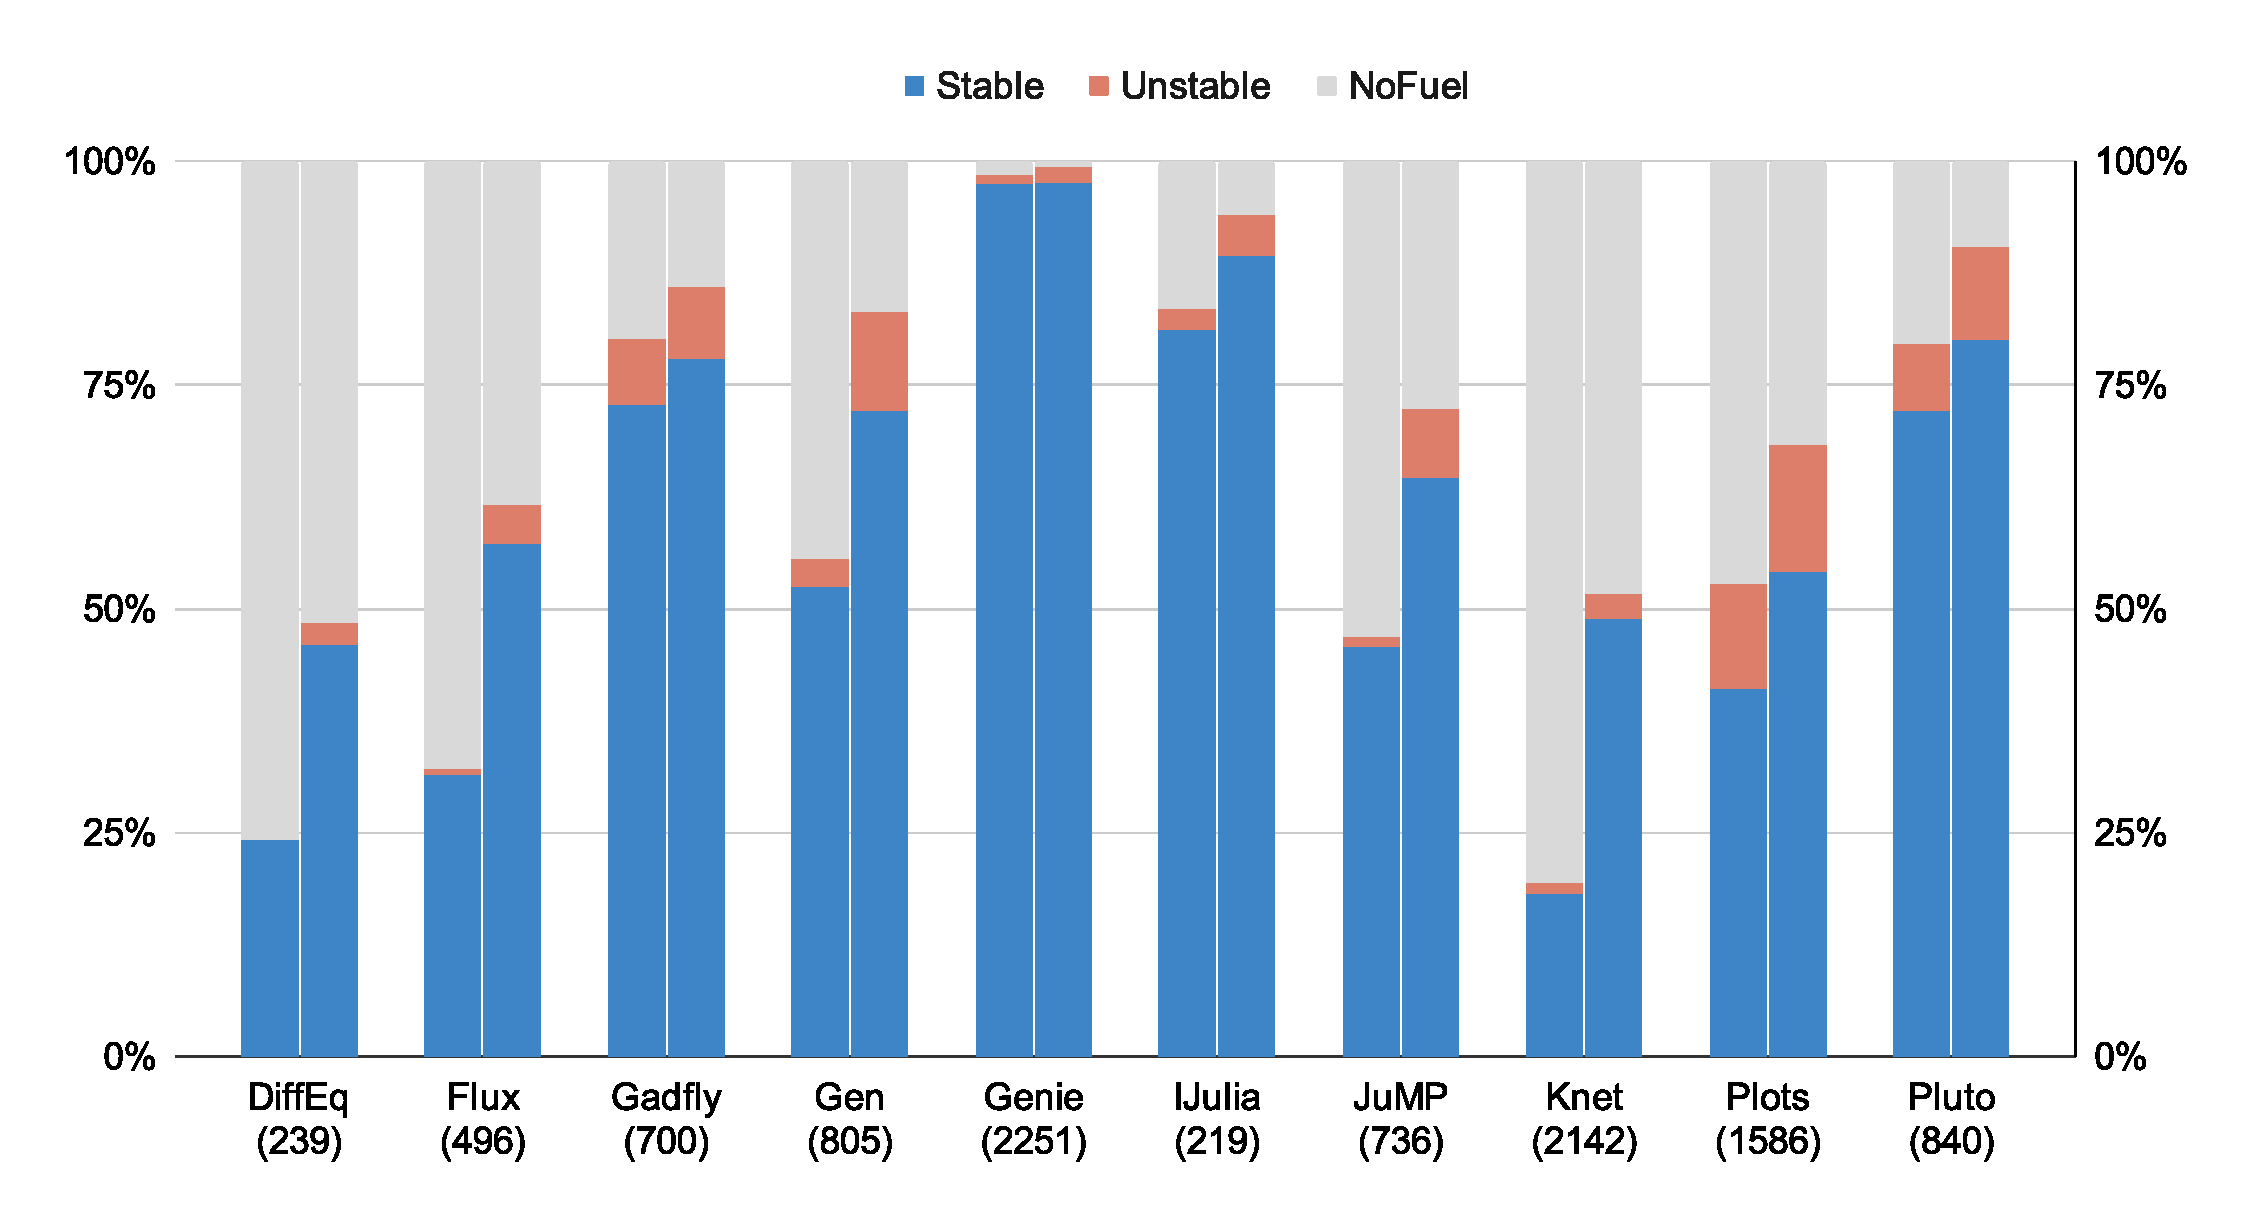
\includegraphics[width=1.5\textwidth]{figs/sts-eval/chart.pdf}
  }
\caption{Inferring Type Stability for the 10 popular Julia packages}%
\label{figs:approx:eval}
\end{figure}

On average over the 10 packages, the analysis identified 54\% of methods as type
stable without sampling, and 69\% of methods as type stable with sampling. The
last figure comes close to the average 72\% of type-stable methods traced via
dynamic analysis. As expected, our static approach is more conservative in granting the
badge because it explores more possibilities for the inputs than what actually
occurs in test suites.

The package having the highest percentage of type-stable methods remains the same as
with the dynamic analysis --- Genie. This is an encouraging result: sometimes static
analysis tools report too many false positive to be viable in practice.
The same is not necessarily an issue with our approach, as
the present analysis of Genie shows: a package that does not have type stability
issues in practice is also reported as such by the tool.

The least type-stable package, according to the dynamic analysis is Knet, and it
is also identifiable on \figref{figs:approx:eval}. The only difference is that
on the figure most of the methods in Knet are marked as \emph{NoFuel} (80\%)
instead of \emph{Unstable}. The \emph{NoFuel} metrics corresponds to the third
of the three possible outcomes listed in \secref{sec:approx:algo-final}. This
result for Knet shows that the \emph{NoFuel} metrics should, perhaps, be
interpreted as \emph{Unstable}, at least, for the packages which we know to have issues
with type stability.

Close to Knet in the amount of methods marked \emph{NoFuel} is
DifferentialEquations (called DiffEq for brevity on the figure), 76\% (24\%
\emph{Stable}), which is a significant difference from the results of dynamic
analysis where it comes as 70\% stable. A probable reason for this is a
considerably different sample of methods analyzed: due to the structural
peculiarities of the package, organized as several subpackages, the current
implementation only processed a portion of methods (namely, those belonging to
one subpackage DiffEqBase). The methods analyzed here constitute about $1/5$ of
methods captured during dynamic analysis. The increase in the number of methods
not identified as type stable is the only significant one (more than 25
percentage points): all other packages has this number increased in less
than 20 percentage points with respect to the results of the dynamic analysis.

Sampling makes the largest difference for packages that have more
\emph{NoFuel}-methods, which is to be expected. Foe example, $20$ or more
percentage points increase in the number of stable methods due to sampling is
found in least type-stable packages: Knet, DifferentialEquations, Gen and Flux.
Unexpected is that finding counterexamples, i.e. increasing
the number of unstable methods, is not always in a rigid correlation with the
number of \emph{NoFuel}-methods. Foe example, adding sampling for DifferentialEquations
(76\% \emph{NoFuel} initially) gives an increase in unstable methods by 3 percentage
points, whereas sampling for JuMP (53\% \emph{NoFuel} initially, just above the median value
of 46\%) gives an increase in unstable methods by 7 percentage points. Adding
sampling does produce non-neglegible number of counterexamples but, perhaps, could
be improved using types databases created specifically to reflect the use cases
of a package under analysis.
